\section{Google Streetview Crawler}
Classification of real-world images requires a very big dataset for the learning process beforehand. Google Streetview provides 360 degree images from many places in all German urban areas. Using sophisticated crawling techniques, a huge amount of image data can be extracted from these, so called, `Photospheres'.\\
This chapter describes how we used the Google Streetview and other image APIs to crawl images from famous sights in Berlin.

\subsection{Image Crawler}
We provide a Google Streetview image crawling python script inside the \texttt{streetviewcrawler} folder. This script takes a csv file as input, which specifies the parameters the crawler needs, such as position and viewing angle. Chapter \ref{csv_file} explains the contents of this file.\\
All requirements for the crawler are specified in the \texttt{requirements.txt} file and can be installed with the command \texttt{\$pip install -r requirements.txt}.\\
Given a location in longitude and latitude, the image crawler will automatically create jpeg-images from different viewing angles. These angles can either be specified or automatically generated by calculating the angle between two geo-coordinates. In the latter case, the script will generate images in five degree steps from 30 degrees to the left to 30 degrees to the right of the calculated viewing angle. If specified by hand, we use one degree steps from the starting to the end angle.\\
Because photospheres can change or get removed, the API uses the closest photosphere to the location provided. This might not be the location specified in the CSV file, which is why we also check the metainformation of each photosphere for the coordinates connected to the image and the status code. In case there is no image in a certain area, the status code tells us that and we don't need to go through all the requests.\\
To prevent Denial-of-Service attacks, the API uses a time- and request-based blocking system. That means, that an IP might be denied further downloads if it either makes request too fast or it reaches the maximum amount. To counter the first blockage, our script uses an exponential wait mechanism. If requests were made too quickly, it waits for a short while before retrying. If it still gets no result, the wait time is increased. This is repeated until the blockage is lifted.\\
For the second part, we provide the usage of a Google API key\footnote{https://developers.google.com/maps/documentation/streetview/}, which can be passed to the crawler script with the \texttt{--key \{key\}} command line switch. The API key enables the crawler to request 25000 requests per day for free, with the option to increase the volume against money.

\subsection{Setup of viewing parameters}\label{csv_file}
The setup CSV file holds all parameters needed for the crawler.

\subsection{State of Automation (i.e. taking one image per viewing angle)}

\subsection{Current Limitations}
Full automation not possible as of current street view API state; wrong latitude/longitude; Streetview Image API returns different images than JavaScript API (which is being used on Google maps website)

\subsection{Possible Improvements}
Use Classifier to identify things in photsphere

\subsection{Google Places API}
For our project, we use several API from Google which help us get mainly two things. Complementary informations about a particular place such as: Name of the place, adresse of the place, phone Number, Web site, rating from Google reviews.
\begin{itemize}
    \item {PLACE DETECTION API}
\end{itemize}
The place detection API will allow us to discover the place near where the device is located. By places, it means all places registered on Google including local businesses, points of interest, and geographic locations. This api will return a maximum of 10 probable places. We can retrieve informations like adresse, phone number or web site.
Another very interesting use is that it can help us determinate if our prediction is relevant, by comparing our classification with the results from this functions.

\begin{itemize}
    \item {GEO DATA API}
\end{itemize}
The Google Places API provides more informations about a place, including the place's reviews and address, the geographical location specified as latitude/longitude coordinates, the type of place (such as night club, pet store, museum) and more. The only constraint is to use a specific place ID from Google, which you can get from the Place detection API.

\begin{itemize}
    \item {How to use it for android}
\end{itemize}
First step, you need to get the api key from Google "https://developers.google.com/?hl=fr". To get the API key, you need to register on the developper console from Google. This platform is the access to every API provide by the firm. Then, you are free to activate any

Second step, you need to declare in the android manifest function your API key between application tag and the first <Activity> tag.

\begin{lstlisting}[language=XML, basicstyle=\scriptsize]
<meta-data
android:name="com.google.android.gms.version" android:value="@integer Google_play_services_version"/>
<meta-data
android:name="com.google.android.geo.API_KEY" android:value="API_KEY"/>
\end{lstlisting}
Then, for the third step, you need to ask permissions in the android manifest for internet and GPS location.
\begin{lstlisting}[language=XML, basicstyle=\scriptsize]
<uses-permission android:name="android.permission.INTERNET"/>
<uses-permission android:name="android.permission.ACCESS_NETWORK_STATE"/>
<uses-permission android:name="android.permission.ACCESS_FINE_LOCATION"/>
\end{lstlisting}

Fourth step, you should declare a "GoogleMapApi" builder and add the several API you want to use. In our case, and illustrate by the following snippet, we use PLACE_DETECTION_API and GEO_DATA_API.

\begin{lstlisting}[language=XML, basicstyle=\scriptsize]
mGoogleApiClient = new GoogleApiClient.Builder(this)
                .addApi(Places.PLACE_DETECTION_API)
                .addApi(Places.GEO_DATA_API)
                .enableAutoManage(this, GOOGLE_API_CLIENT_ID, this)
                .build()
\end{lstlisting}

For the final step, it's calling the function. You need to use the "Places" package associate with the api you want to use. Then the most important thing is to add your Google api builder as a parameter of the function.
\begin{lstlisting}[language=XML, basicstyle=\scriptsize]
#For the PLACE DETECTION API
Places.PlaceDetectionApi.getCurrentPlace(mGoogleApiClient, null);

#For the GEO DATA API
Places.GeoDataApi.getPlaceById(mGoogleApiClient, placeId)
\end{lstlisting}

\begin{itemize}
    \item {Limitations}
\end{itemize}

Google provide a really useful and powerful service but the only constraint is the limitation. We can only have 1,000 free requests per 24 hour period, which is already great but not for a multiple user application.
Therefore, they provide a business API plan that can be adapte if needed which give access to 150 000 request per day and can be increased more depending on the number of requests needed.

\subsection{Shutterstock/Flickr and Pinterest}

Shutterstock/flickr and Pinterest are public web application for hosting and sharing photos and images. For exemple on Flickr nearly 7,000 photos are uploaded per minute.
As these services are used by both professional and amateurs photographers, we can find a lot of great and good quality images.
It's easy to create an API key, just register on the web site of each applications.


\begin{itemize}
    \item {Exemple to get images URL}
\end{itemize}
Our exemple for getting Image url which can be downloaded after use angularJs API package and store them into a mongoDb database.

First we declare variable for our api connection
\begin{lstlisting}[language=XML, basicstyle=\scriptsize]
var api = shutter.v2({
    clientId: 'Your public key',
    clientSecret: 'Your secret key',
});
\end{lstlisting}
Then we detail the search string we want to crawl.Here we choose the Branderburg gate.
\begin{lstlisting}[language=XML, basicstyle=\scriptsize]
var opts = {
    query: 'Brandenburg',
    page: 1,
    per_page: 200,
    sort : 'popular'
};
\end{lstlisting}
Finally, we navigate through the json response to get the url.
\begin{lstlisting}[language=XML, basicstyle=\scriptsize]

    api.image.search(opts, function(err, data) {
        if (err) throw err;

        console.log(data.data[0].id);
        var arrayLenght = data.data.length;
        console.log(arrayLenght);

        for (var i = 0; i < arrayLenght; i++) {

        var obj = data.data[i];
        console.log(obj);
        }
\end{lstlisting}
The response return will be as follow.\\
\\
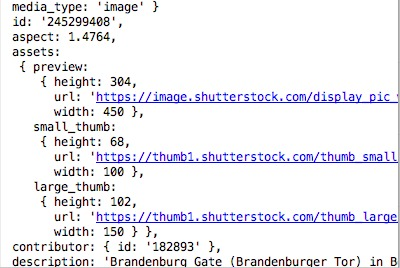
\includegraphics{jsonShutter}
\begin{itemize}
    \item {Limitations}
\end{itemize}
These services are limited to 3600 call per hours. And your API key can be block if the service detect an abuse use of the service.
